\documentclass{standalone}
\usepackage{tikz}
\begin{document}
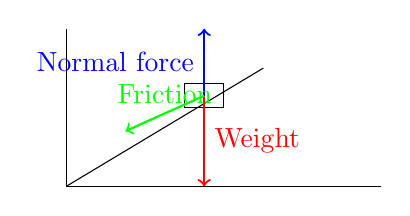
\begin{tikzpicture}
    % Draw inclined plane
    \draw (4,0) -- (0,0) -- (0,2);
    \draw (0,0) -- (2.5,1.5); % inclined plane
    % Draw rectangle (object)
    \draw (1.5,1) rectangle (2,1.3);
    % Draw forces
    \draw[->,red,thick] (1.75,1.15) -- (1.75,0) node[midway,right] {Weight}; % weight
    \draw[->,blue,thick] (1.75,1.15) -- (1.75,2) node[midway,left] {Normal force}; % normal force
    \draw[->,green,thick] (1.75,1.15) -- (0.75,0.7) node[midway,above] {Friction}; % friction
\end{tikzpicture}
\end{document}